%\vspace{-2pt}
\subsection{Experiment Setup}
\label{subsec:res-setup}

In the analytic evaluation, the target MAAR platform settings \newtext{are: (1) An ARM CortexA57 processor with} 4 ARMv8-A cores simulated at the 1.4GHz clock frequency, analytic computing performance of each core is 2000 MIPS. (2) A multi-layer AMBA AHB (32 bit-width, 200MHz) with eight concurrent channels (4R and 4W). (3) Four DMA modules. (4) A shared 8MB memory module with four access ports. (5) The processing speed up on ACCs is varied depending on the parallelization of each kernel. (6) ACCs can communicate directly with each other~\cite{teimouri2016improving}. 

For energy estimation, \newtext{the analytic model assumes 14pJ per 8 bytes data transfer \cite{keckler2011gpus}, 3.8pJ for each kilo operations in the ACCs \cite{cong2014accelerator}, 800mW power for each ARM core running at 1.4GHz \cite{ARMcorePower},} and 30mW static power per each 100KB of on-chip shared memory \cite{malladi2012towards}.

Allocate one MAAR platform for 40 OpenVX applications captured in annotated dataflow. 
They are real vision applications found in \cite{Intel}, \cite{AMD}. 
The number of processing kernels in applications ranges from 3 to 14, and the number of edges/links varies is from 2 to 17. 
The applications are composed of 35 types of unique processing kernels.
Each kernel can be instantiated at most once in HW, and multiple instances are scheduled sequentially.

\begin{figure}[h]
\vspace{-8pt}
	\centering
		\subfloat[MAAR and DSS] {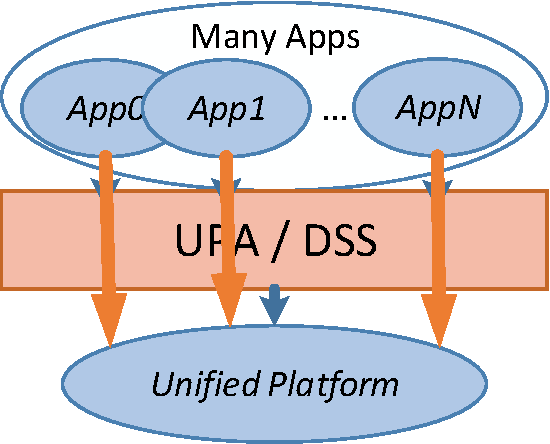
\includegraphics[width=.28\linewidth]{fig/DSSMAAR.pdf}\label{fig:mapMAAR}}
		\hfill
		\subfloat[1AppDSE] {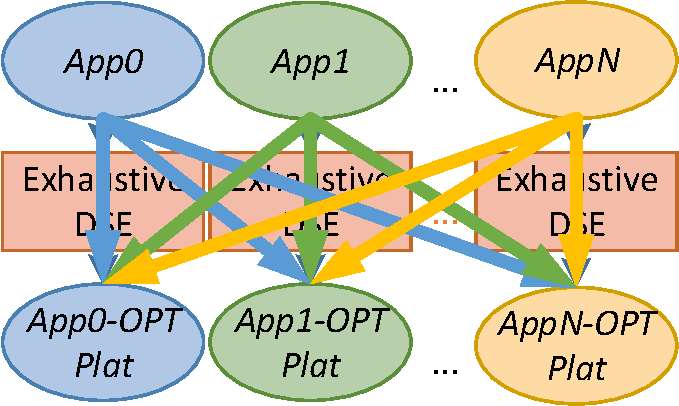
\includegraphics[width=.32\linewidth]{fig/FOP.pdf}\label{fig:mapFOP}}
		\hfill
		\subfloat[OOP] {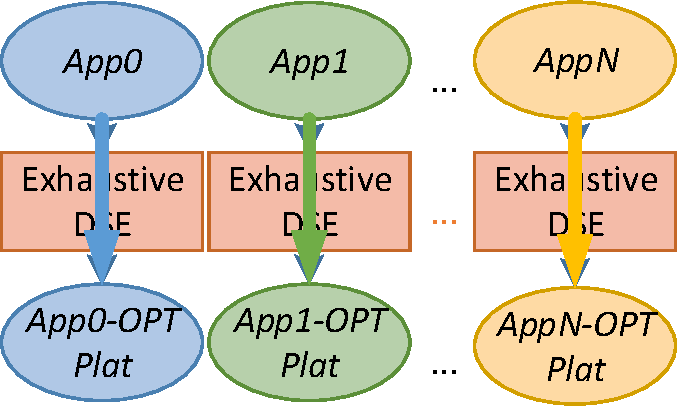
\includegraphics[width=.32\linewidth]{fig/OOP.pdf}\label{fig:mapOOP}}
	\vspace{-8pt}
	\caption{Experiments Settings}
	\label{fig:avg}
\end{figure}

To understand the benefits of MAAR Evaluation, this section compares MAAR DSE with DSS~\cite{zhang2018ds} and 1AppDSE. \newtext{As \figref{fig:mapMAAR} shown, both MAAR and DSS platform is designed for many applications. DSS is a greedy algorithm for platform allocation according to characteristics analysis across applications without an evaluation. While in \figref{fig:mapFOP},} 1AppDSE considers one application in isolation instead of many applications. In the experiments, an exhaustive search is used to find the 1AppDSE platform, which gives the optiamal (OPT) platform for one application. Then mapping all applications on this platform provides one 1AppDSE platform performance. To get the average performance of 1AppDSE, this paper maps all applications onto all OPT platforms (one platform from one application). Similar to OOP, 1AppDSE results in the same number of platforms. However, \newtext{OOP in \figref{fig:mapOOP} only maps the application on its Own Optimal Platform (OOP), while 1AppDSE maps all applications onto each platform.}

\begingroup
\setlength{\columnsep}{8pt}%
\begin{wrapfigure}{l}{0.5\linewidth}
	%\vspace{-6pt}
	\begin{center}
		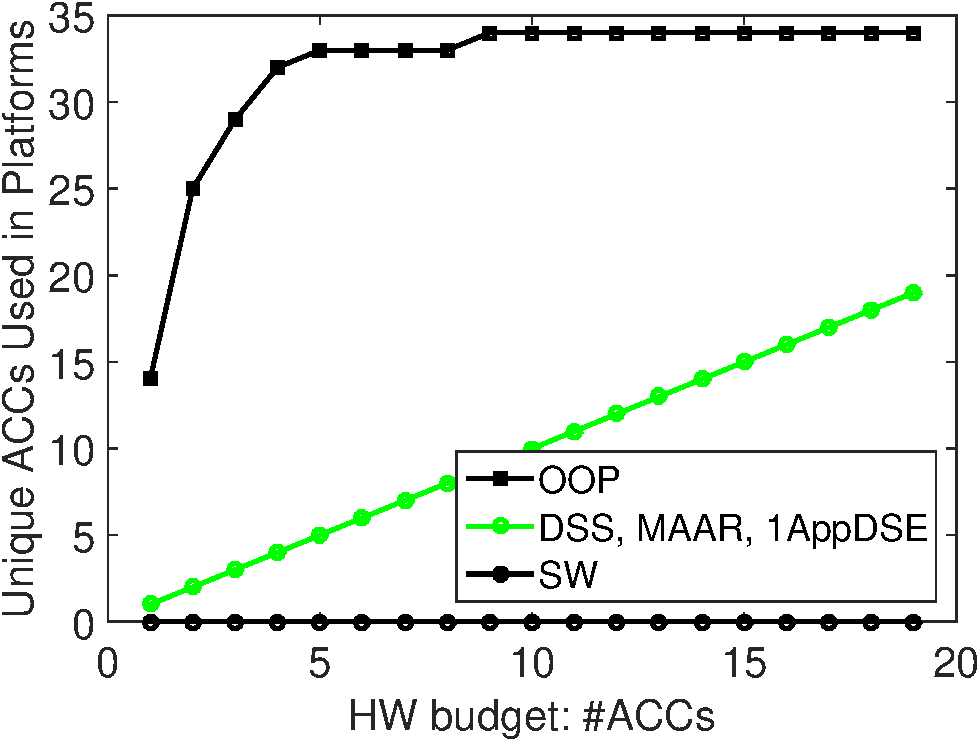
\includegraphics[width=\linewidth]{fig/oopHW.pdf}
	\end{center}
	%\vspace{-8pt}
	\caption{Unique ACCs Used in Platform(s)}
	\label{fig:oopHW}
	%\vspace{-4pt}
\end{wrapfigure}


\figref{fig:oopHW} lists the number of unique ACCs \newtext{ in platform(s) for each DSE}
(SW is empty; DSS, MAAR and 1AppDSE are equal to the budget). OOP has one platform per application, so there are 40 platforms for all applications. Each OPT platform has a number of ACCs equal to the budget, so there are a large number of unique ACCs \newtext{for all OPT platforms}. When each OPT platform has 1 ACC, there are 14 unique ACCs, indicating some reuse. However, if each OPT platform has 2 ACCs, there are 25 unique ACCs (11 more) showing the limits of reuse. 

\endgroup